\documentclass{article}

\usepackage{a4}
\usepackage{amsmath}
\usepackage{amssymb}
\usepackage{ctex}
\usepackage{booktabs}
\usepackage{graphicx}
\usepackage{subfigure}
\usepackage{subcaption}
\usepackage{float}
\usepackage{hyperref}
\usepackage{xurl}
\usepackage{enumitem}
\usepackage{array}
\usepackage{longtable}
\usepackage{multirow}
\usepackage{fvextra}

\hypersetup{colorlinks=true,linkcolor=black,urlcolor=blue,citecolor=black}
\setlist[itemize]{nosep,leftmargin=1.8em}
\setlist[enumerate]{nosep,leftmargin=1.8em}
\captionsetup{font=small}
\setlength{\emergencystretch}{3em}
\renewcommand{\arraystretch}{1.2}
\RecustomVerbatimEnvironment{verbatim}{Verbatim}{
  breaklines=true,
  breakanywhere=true,
  fontsize=\small
}
\newcommand{\sourcecode}[2]{
  \subsubsection*{#1}
  \noindent 对应文件：\path{#2}
  \VerbatimInput[
    breaklines=true,
    breakanywhere=true,
    fontsize=\small
  ]{#2}
}

\title{计算机组成原理 Project1 实验报告（Week 1）\\8位定点卷积--激活--池化链运算器设计}
\author{鲁昕宁 2414015}
\date{\today}

\begin{document}

\maketitle
\begin{center}
  \url{https://github.com/SidneyLu/Computer-Organization-and-Design-NKU-CS/tree/master/project1}
\end{center}

\newpage

\section{实验目标}
本实验面向边缘端 AI 场景，设计并验证一个 8 位定点卷积--激活--池化链运算器。工程目标如下：
\begin{itemize}
  \item 输入为 $5\times 5$ 的 8 位无符号灰度矩阵，像素范围为 $0\sim255$；
  \item 运算流程为 ``$5\times 5$ 输入 $\rightarrow$ $3\times 3$ 卷积层 $\rightarrow$ ReLU 激活层 $\rightarrow$ $2\times 2$ 平均池化层''；
  \item 输出为 $2\times 2$ 的 8 位特征值矩阵；
  \item 在 Vivado 环境下完成模块设计、功能仿真、综合与时序分析，并比较不同优化方案的资源占用与性能。
\end{itemize}

\section{实验环境}
本工程的开发与验证环境如下：
\begin{itemize}
  \item FPGA 器件：Xilinx Artix-7 \texttt{xc7a200tfbg676-2}
  \item RTL 语言：Verilog HDL
  \item 功能仿真：Vivado 2025.1 / XSIM
  \item 综合与时序分析：Vivado 批处理脚本 \texttt{scripts/run\_vivado\_multi\_synth.tcl}
  \item 时钟约束：\texttt{create\_clock -period 5.000 -name clk [get\_ports clk]}，即 200\,MHz
  \item I/O 约束：\texttt{set\_input\_delay 0.000} 与 \texttt{set\_output\_delay 0.000}
\end{itemize}

波形保留策略也在工程中固化：
\begin{itemize}
  \item XSIM 原始波形数据库保存在 \verb|build/xsim/waves/*.wdb|；
  \item 便于二次处理的文本波形保存在 \verb|build/xsim/waves/*.vcd|；
  \item 报告中的代表性波形图由 \verb|scripts/export_wave_figures.py| 从 VCD 自动导出到 \verb|report/figures/|。
\end{itemize}

\section{实验原理}
\subsection{卷积运算}
输入图像记为 $X$，卷积核记为 $K$。本实验采用 $3\times 3$ 卷积核对 $5\times 5$ 输入做 valid 卷积，得到 $3\times 3$ 特征图：
\[
Y(i,j)=\sum_{u=0}^{2}\sum_{v=0}^{2} X(i+u,j+v)\cdot K(u,v),\quad 0\le i,j\le 2
\]
其中像素 $X(i,j)$ 为 8 位无符号数，卷积核权重 $K(u,v)$ 为 8 位有符号数。

\subsection{ReLU 激活}
卷积输出经过 ReLU 激活后，负数被截断为 0，正数保留：
\[
R(i,j)=\max(0,Y(i,j))
\]
为保证最终结果能安全落回 8 位无符号范围，本工程进一步加入上饱和处理：若 $R(i,j)>255$，则输出钳位为 255。

\subsection{平均池化}
对 $3\times 3$ 激活图执行 $2\times 2$ 平均池化，输出 $2\times 2$ 结果：
\[
P(i,j)=\left\lfloor \frac{R(i,j)+R(i,j+1)+R(i+1,j)+R(i+1,j+1)}{4}\right\rfloor,\quad 0\le i,j\le 1
\]
由于分母恒为 4，硬件上可直接用右移 2 位实现，因此无需额外的通用除法器。

\subsection{实验分组}
本次实验实现了 5 个独立顶层：
\begin{enumerate}
  \item 串行：\texttt{cnn\_compare\_base\_top}
  \item 串行 + BoothWallace 乘法器优化：\texttt{cnn\_compare\_booth\_top}
  \item BoothWallace 乘法器优化 + SIMD：\texttt{cnn\_compare\_booth\_simd\_top}
  \item BoothWallace 乘法器优化 + SIMD + 流水线：\texttt{cnn\_compare\_booth\_simd\_pipe\_top}
  \item 第 4 组基础上换用 DSP：\texttt{cnn\_compare\_booth\_simd\_pipe\_dsp\_top}
\end{enumerate}

\section{里程碑1：核心模块设计与功能验证}
\subsection{基础模块设计}
里程碑 1 首先完成了 4 个基础模块的串行版本：
\begin{itemize}
  \item \texttt{mul8}：8 位无符号像素与 8 位有符号卷积核的乘法；
  \item \texttt{add8}：8 位无符号加法；
  \item \texttt{relu\_s20}：20 位有符号卷积结果的 ReLU 与 8 位饱和截断；
  \item \texttt{div4}：10 位无符号数除以 4 的右移实现。
\end{itemize}

下面在模块首次介绍的位置给出对应的完整 Verilog 源码。

\sourcecode{模块 \texttt{mul8} 的 Verilog 源码}{../src/baseline/mul8.v}
\sourcecode{模块 \texttt{add8} 的 Verilog 源码}{../src/baseline/add8.v}
\sourcecode{模块 \texttt{relu\_s20} 的 Verilog 源码}{../src/baseline/relu_s20.v}
\sourcecode{模块 \texttt{div4} 的 Verilog 源码}{../src/baseline/div4.v}

在此基础上，又按计划补齐了优化所需模块：
\begin{itemize}
  \item \texttt{mul8\_booth\_wallace}：真实的基 4 Booth 编码 + Wallace 树压缩 8 位乘法器；
  \item \texttt{simd\_mul8x4}：4 路 BoothWallace lane 封装；
  \item \texttt{simd\_add8x4}、\texttt{simd\_relu8x4}、\texttt{simd\_avgpool2x2\_8bit}：分别承担 4 路加法、4 路激活与池化求均值；
  \item \texttt{simd\_mul8x4\_dsp} 与 \texttt{mul8\_dsp48e1}：作为第 5 组 DSP 版的乘法实现。
\end{itemize}

优化模块源码与仿真结果详见第三部分。

\subsection{模块级仿真}
本实验所有仿真均通过 Vivado XSIM 完成。统一命令为：
\begin{verbatim}
powershell -ExecutionPolicy Bypass -File .\scripts\run_vivado_sim.ps1 -Mode all
\end{verbatim}

其中基础模块验证可单独使用：
\begin{verbatim}
powershell -ExecutionPolicy Bypass -File .\scripts\run_vivado_sim.ps1 -Mode basic
\end{verbatim}

模块级 testbench 的覆盖范围如表 \ref{tab:tb-basic} 所示。

\begin{table}[H]
\centering
\caption{里程碑 1 模块级 testbench}
\label{tab:tb-basic}
\begin{tabular}{lll}
\toprule
testbench & 验证对象 & 覆盖方式 \\
\midrule
\texttt{tb\_mul8} & \texttt{mul8} & 穷举 65536 组 ``像素$\times$权重'' 输入 \\
\texttt{tb\_add8} & \texttt{add8} & 穷举 65536 组 8 位无符号加法输入 \\
\texttt{tb\_relu\_s20} & \texttt{relu\_s20} & 负数、线性区间、饱和区间与边界值 \\
\texttt{tb\_div4} & \texttt{div4} & 穷举全部 1024 组 10 位输入 \\
\bottomrule
\end{tabular}
\end{table}

Vivado 日志显示上述 testbench 均通过：
\begin{itemize}
  \item \texttt{tb\_mul8 PASS}
  \item \texttt{tb\_add8 PASS}
  \item \texttt{tb\_relu\_s20 PASS}
  \item \texttt{tb\_div4 PASS}
\end{itemize}

按照验证对象顺序，下面给出里程碑 1 的基础模块 testbench 源码。
\sourcecode{testbench \texttt{tb\_mul8} 的 Verilog 源码}{../sim/tb_mul8.v}
\sourcecode{testbench \texttt{tb\_add8} 的 Verilog 源码}{../sim/tb_add8.v}
\sourcecode{testbench \texttt{tb\_relu\_s20} 的 Verilog 源码}{../sim/tb_relu_s20.v}
\sourcecode{testbench \texttt{tb\_div4} 的 Verilog 源码}{../sim/tb_div4.v}

优化模块的 testbench（\texttt{tb\_mul\_compare}、\texttt{tb\_simd\_mul\_compare}）源码与仿真结果详见第三部分。

\subsection{代表性基础模块波形}
下面给出 4 个基础模块的代表性波形，按模块验证顺序依次展示。

\begin{figure}[H]
  \centering
  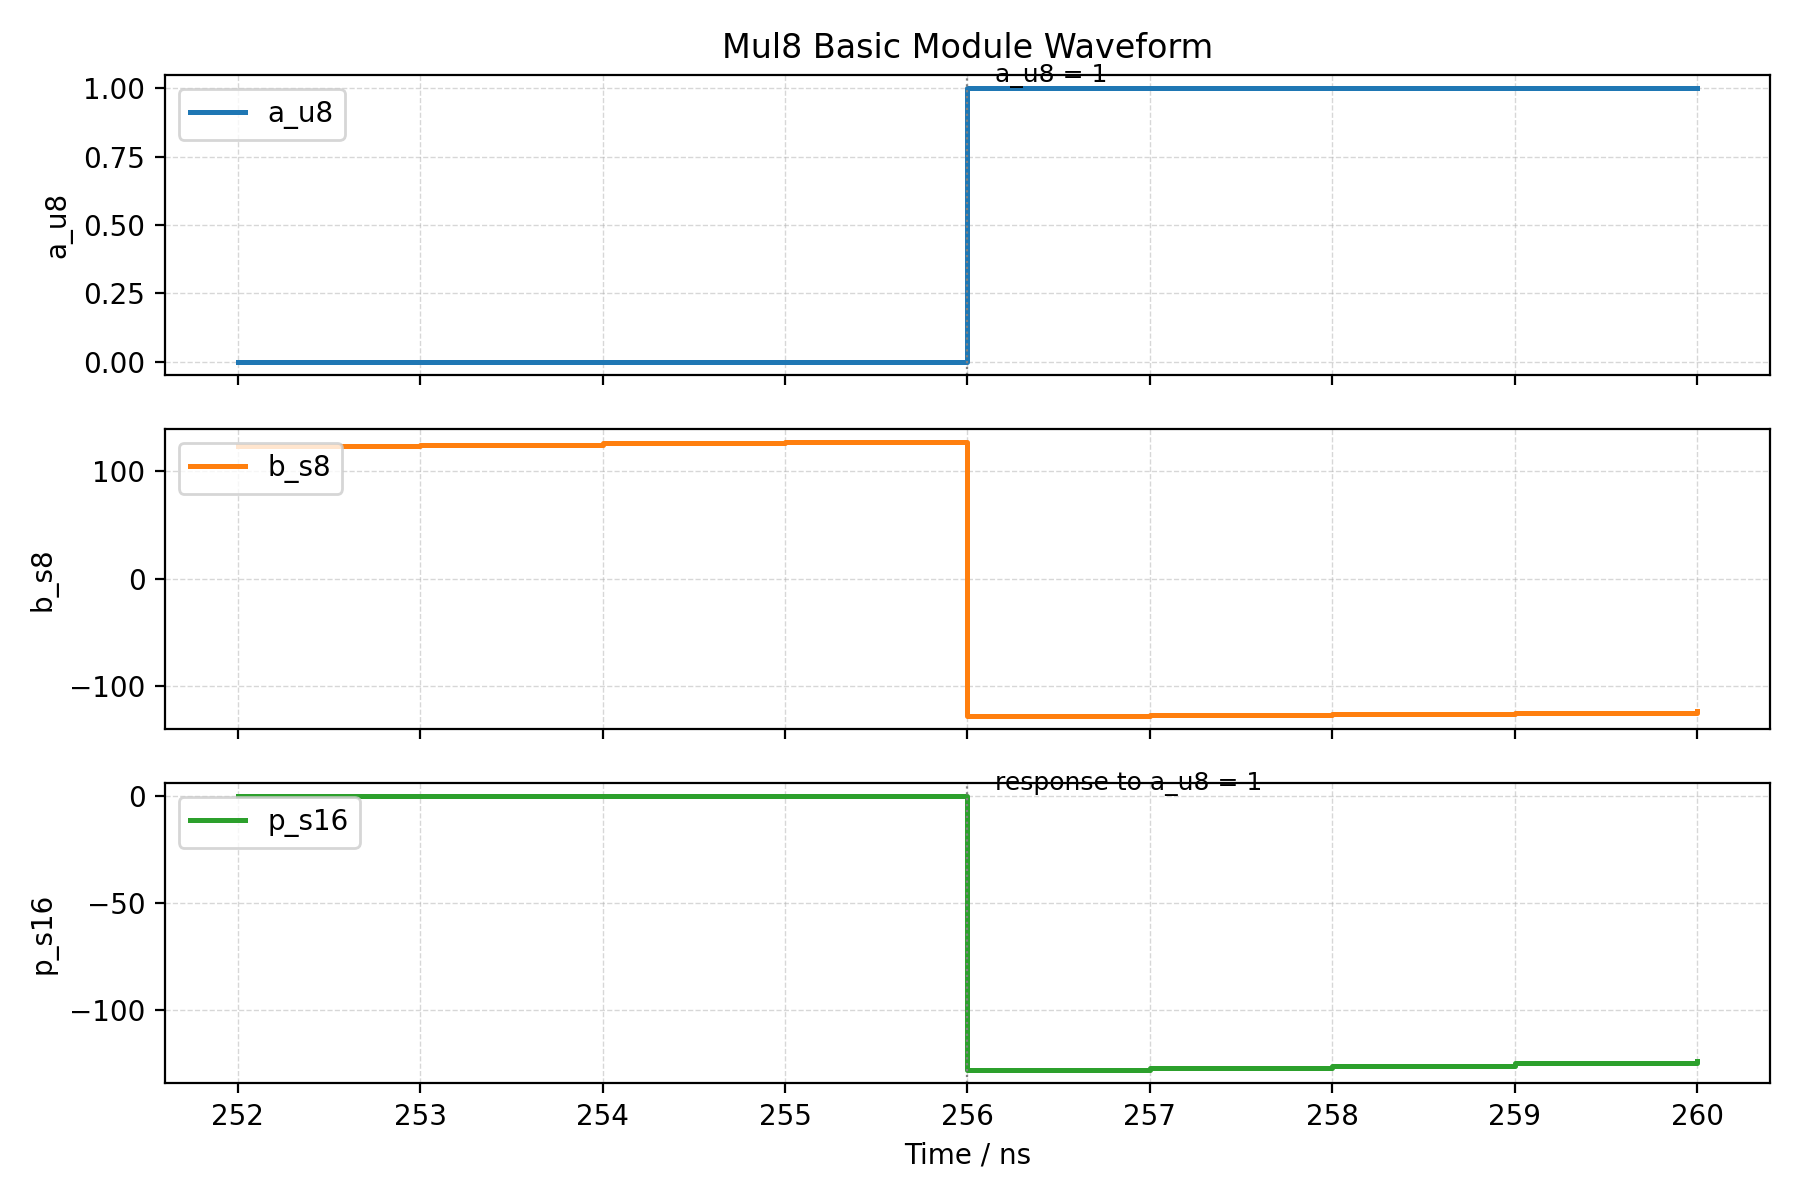
\includegraphics[width=0.92\textwidth]{figures/wave_mul8_basic.png}
  \caption{基础模块波形：\texttt{mul8} 的乘法响应}
  \label{fig:wave-mul8}
\end{figure}

\begin{figure}[H]
  \centering
  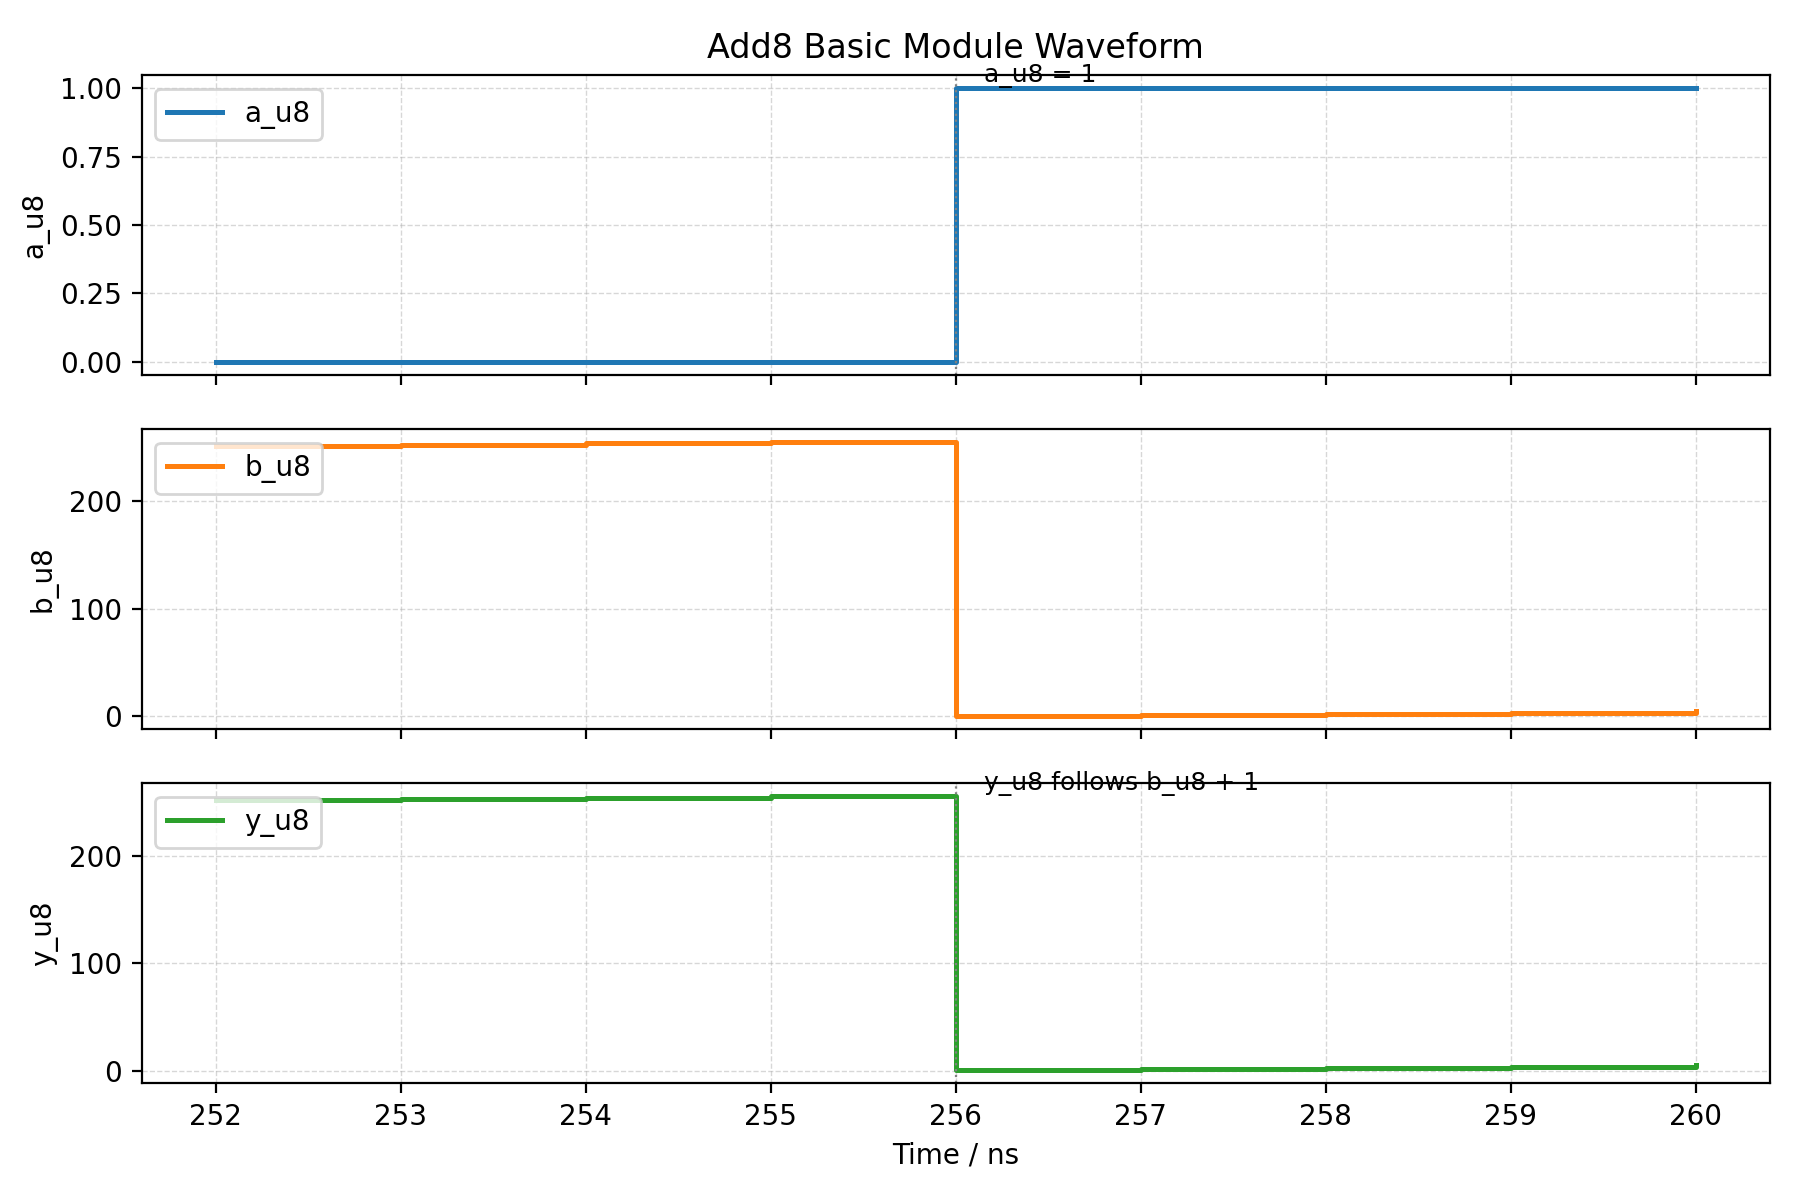
\includegraphics[width=0.92\textwidth]{figures/wave_add8_basic.png}
  \caption{基础模块波形：\texttt{add8} 的加法响应}
  \label{fig:wave-add8}
\end{figure}

\begin{figure}[H]
  \centering
  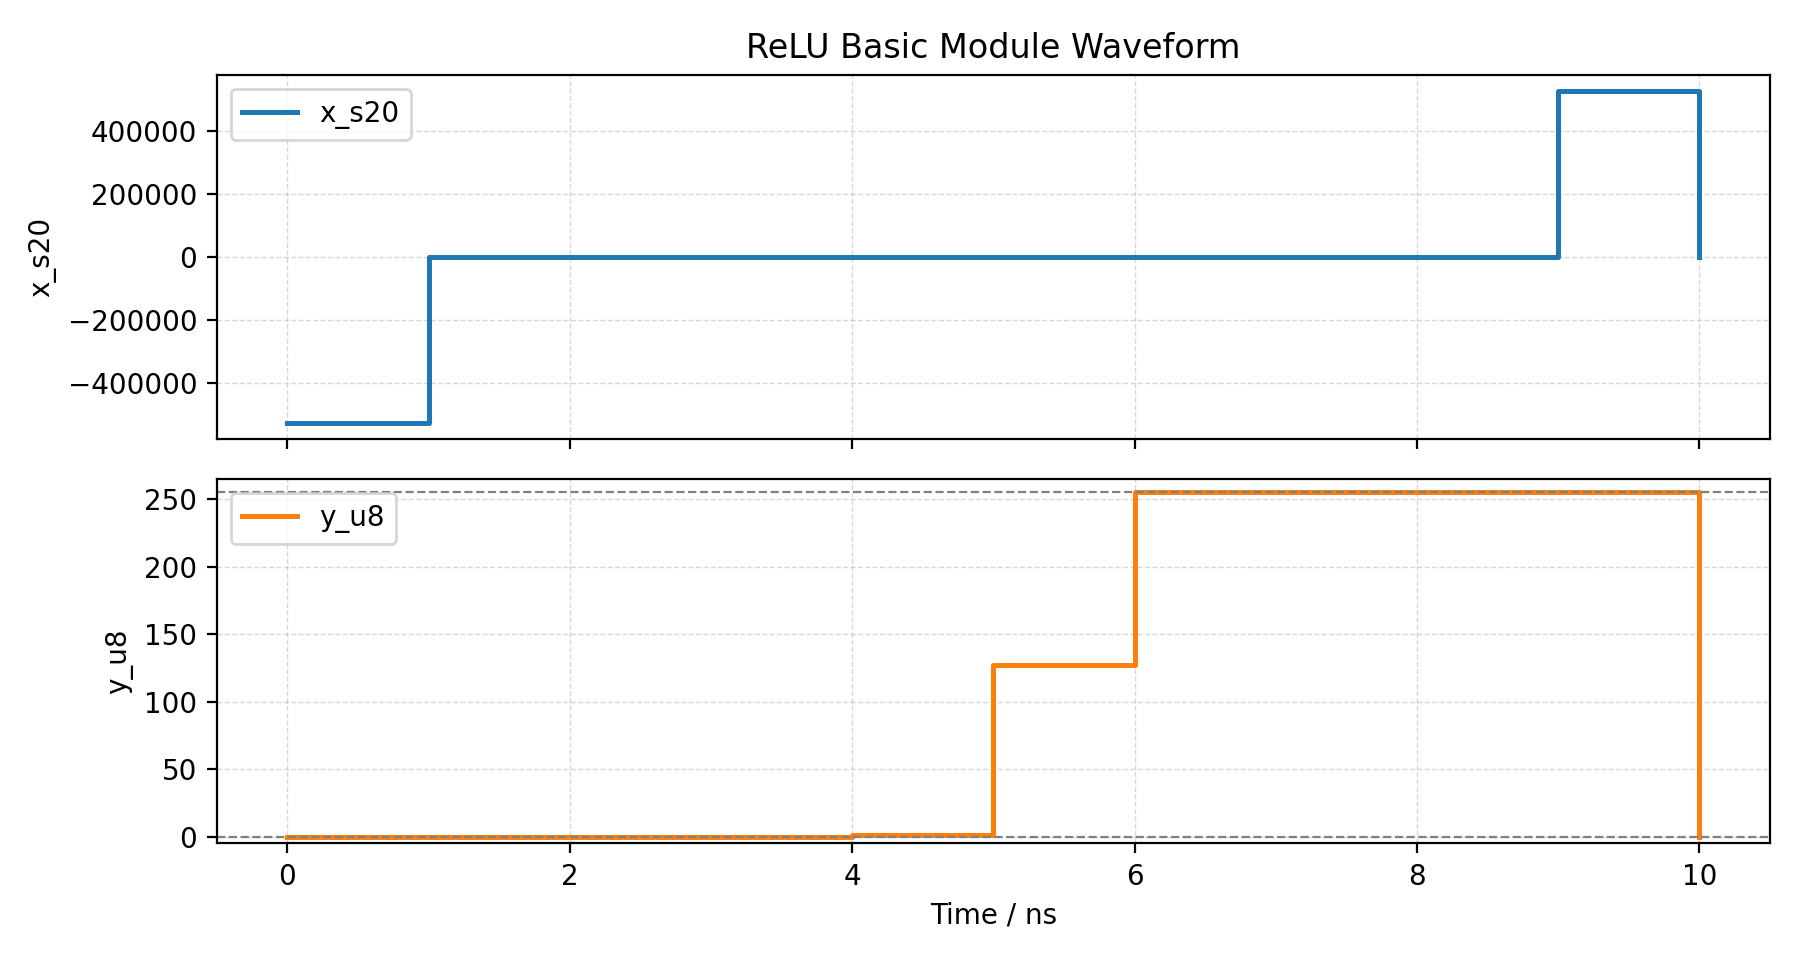
\includegraphics[width=0.92\textwidth]{figures/wave_relu_basic.png}
  \caption{基础模块波形：\texttt{relu\_s20} 的截断与饱和行为}
  \label{fig:wave-relu}
\end{figure}

\begin{figure}[H]
  \centering
  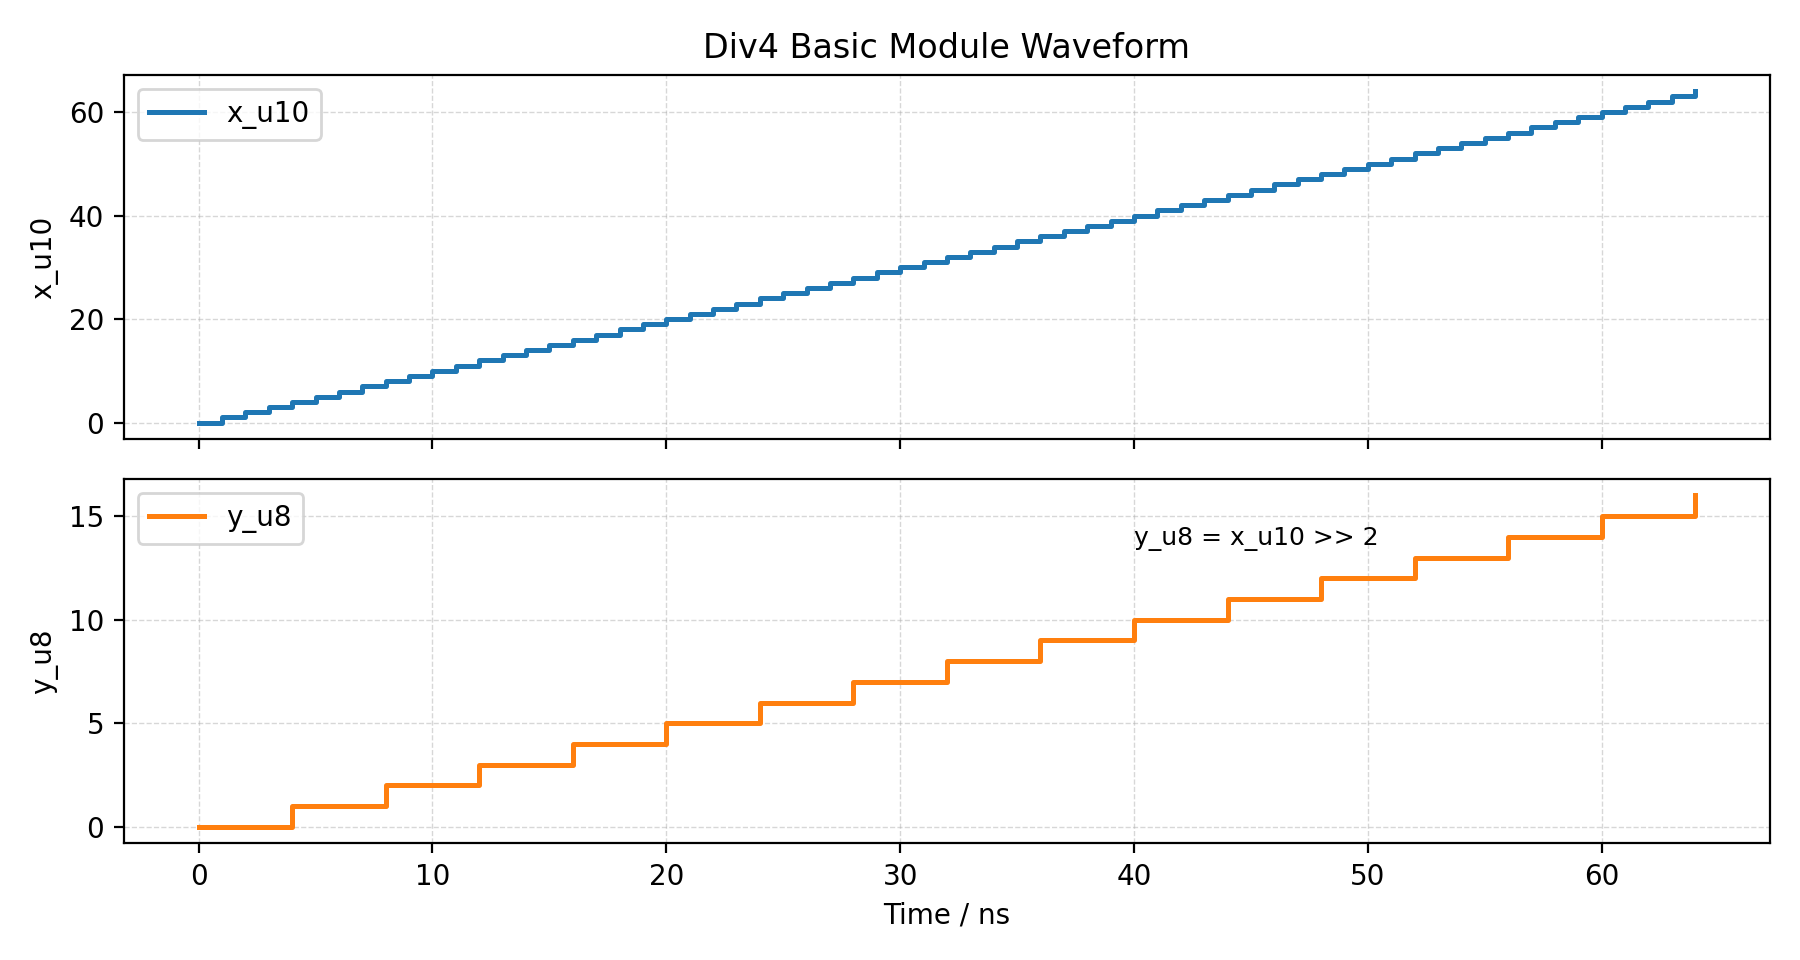
\includegraphics[width=0.92\textwidth]{figures/wave_div4_basic.png}
  \caption{基础模块波形：\texttt{div4} 的右移除 4 行为}
  \label{fig:wave-div4}
\end{figure}

\end{document}
